%%%%%%%%%%%%%%%%%%%%%%%%%%%%%%%%%%%%%%%%%%%%%%%%%%%%%%%%%%%%%%%%%%%%%%%%%%%%%%%%%%%%%%%%%%%%%
%%									Chapitre 2											%
%%%%%%%%%%%%%%%%%%%%%%%%%%%%%%%%%%%%%%%%%%%%%%%%%%%%%%%%%%%%%%%%%%%%%%%%%%%%%%%%%%%%%%%%%%%%%
\chapter{Stochastic Multi-Armed Bandits}\label{CHAP:MAB}
	\citationChap{
	blabla
	}{}
	\minitoc
	\newpage

%%%%%%%%%%%%%%%%%%%%%%%%%%%%%%%%%%%%%%%%%%%%%%%%%%%%%%%%%%%%%%%%%%%%%%%%%%%%%%%%%%%%%%%%%%%%%

\section{The Multi-Armed Bandits Model}\label{sec:mab.model}

The problem of sequentially allocating resources to a defined set of actions (arms) based on successive \emph{partially observable} (see Definition~\ref{def:mab.mab} and Remark~\ref{remark:mab.partial} below) feedback refers to the MAB game in probability theory. The term \emph{bandit} is named, by analogy, after slot machines (or one-armed bandits) in a casino. A sequential decision making problem comes up then when facing with several slot machines (multi-armed bandits).

The study of MAB problems can date back to as early as 1933~\citep{thompson1933}, and was originally proposed to model sequential clinical trials. For example, researchers testing the efficacy of potential vaccines for a new coronavirus have to choose a vaccine (arm) from the following 4 options as shown in Fig.~\ref{fig:mab.covid} on each patient from an experimental group of $N$ person. For each patient $n\in[N]$, researchers receive a reward signal $r_n\in\{0,1\}$. $r_n=1$ indicates that the vaccine is effective, otherwise the vaccine fails. We thus assume that the efficacy of each vaccine follows some Bernoulli distribution that is unknown to the researchers.

\begin{figure}[ht]
    \centering
    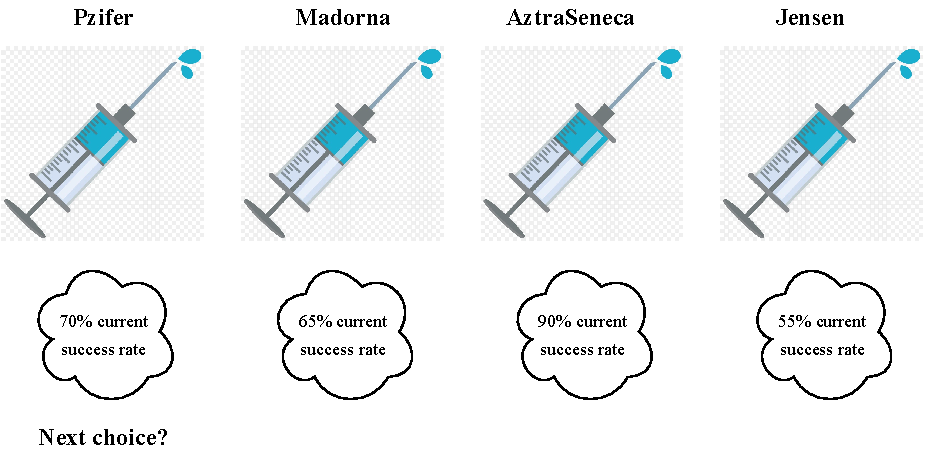
\includegraphics[width=\textwidth]{Chapter2/img/covid.pdf}
    \caption{An example of modelling clinical trials as a MAB problem.}
    \label{fig:mab.covid}
\end{figure}

As stated in Chapter~\ref{CHAP:INTRO}, a common learning objective for stochastic MAB is to maximize the total reward obtained given a sequence of observations. In the previous example, researchers need to decide which vaccine to employ for each patient depending on the previous success rates with the purpose of maximizing the total success rate $\sum_{n=1}^N r_n$ at the end.

However, due to the complex nature of medical treatment, it turns out that the MAB model is hardly applied in real clinical trials despite its primary purpose~\citep{reda2020drug}. Nevertheless, the model has been widely employed in many other applications recently, in particular online recommender systems for example (see e.g.~\citealt{li2010contextual,zeng2016online}). Other application scenarios include network routing~\citep{talebi2018osp}, dynamic pricing~\citep{zhai2011pricing}, demand and supply management~\citep{bregere2019contextual}, sensor placement~\citep{grant2019sensors}, auction bidding~\citep{cesa-bianchi2015auction}, wireless communications in Internet of Things~\citep{besson2019thesis}, etc. 

Those applications sometimes give birth to new variants of \gls{mab}. One of the most studied variants is contextual bandits for which the average reward depend on some external context (see e.g.~\citealt{li2010contextual,krause11contextual}). Linear bandits (see e.g.~\citealt{abbasi-yadkori2011linear}) that we study further in detail in this thesis is typically a particular case of contextual bandits. Other variants include combinatorial bandits in which a subset of arms can be selected at each round (see e.g.~\citealt{cesa-bianchi2012combinatorial,perrault2020semi,chen2014combinatorial}); structured bandits for which prior knowledge on the structure of the arm means is available (see e.g.~\citealt{karnin2016structure,degenne2020structure}); adversarial bandits where the payoffs are controlled by a stochastic process, but rather by a (potentially oblivious) adversary (see e.g.~\citealt{auer2002exp3}); non-stationary bandits where the rewards are changing over time (see e.g.~\citealt{mellor2013nonstationary,allesiardo2017nonstationary}); multi-player bandits for which several learners exist and need to take decisions at some pre-defined moments (see e.g.~\citealt{besson2018multiplayer}); dueling bandits for which the rewards are implicit pairwise comparison results (see e.g.~\citealt{komiyama2015}); delayed bandits where the rewards of current actions are not available immediately (see e.g.~\citealt{vernade2017stochastic}) and so on and so forth.

In the next, we go a little beyond the intuition and provide the formal definition of the model. We also recall some fundamental results for the sake of self-containedness. Of course, we do not intend to write a survey of MAB, for which the content is far too rich for this thesis. Interested readers can refer to~\cite{bubeck2012bandits,lattimore2018bandits} or~\cite{slivkins2019bandits} for further readings and more general results.

\subsection{Problem Formulation}\label{sec:mab.model.formulation}

From a mathematical point of view, a MAB model is a collection of $K$ \emph{unknown} probability distributions $(\nu_k)_{1 \leq k \leq K}$. At each time step $n$, the learner chooses a distribution $\nu_{I_n}$ where $I_n\in[K]$ and receive a reward $r_n$ that is generated from $\nu_{I_n}$. We then recover the bandit learning cycle as shown in Fig.~\ref{fig:mab.mab}. We summarize such a sequential learning procedure in Definition~\ref{def:mab.mab}.

\begin{figure}[ht]
    \centering
    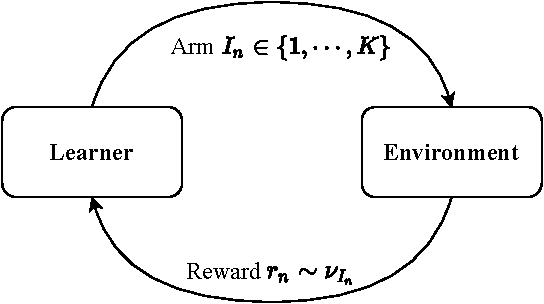
\includegraphics[width=0.5\textwidth]{Chapter2/img/mab_bis.pdf}
    \caption{A bandit learning cycle.}
    \label{fig:mab.mab}
\end{figure}

\begin{definition}[multi-armed bandit game]\label{def:mab.mab}
\begin{leftbar}[defnbar]
	We are given a set of $K$ arms $\{1,\cdots,K\}$ that follow $K$ unknown distributions $(\nu_k)_{1 \leq k \leq K}$, and a time horizon $N$. At each stage $n\in\NN$, the bandit game consists of the following steps:
	\begin{itemize}
		\item a vector of rewards $(r_{n,1} \sim \nu_1, \cdots, r_{n,K} \sim \nu_K)$ is generated,
		\item the learner picks an arm $I_n \in \{1,\cdots,K\}$, and
		\item the learner observes the reward $r_n \eqdef r_{n,I_n}$.
	\end{itemize}
\end{leftbar}
\end{definition}

\begin{remark}\label{remark:mab.partial}
\begin{leftbar}[remarkbar]
	Rewards of unchosen arms at time $n$ are not revealed, this partial feedback setting is a special case of the online learning with experts setting.
\end{leftbar}
\end{remark}

The way that the learner chooses the arm to pull is sometimes called a \gls{sampling rule} or \emph{sampling strategy}. Clearly, the sampling rule should make use of the past observations as well as the past external randomness if present. A very simple way to understand this intuition is to consider a bandit model with two arms with $\mu_1=1, \mu_2=0$. Suppose that the rewards are deterministic. In this case, if we consider a naive sampling strategy that uniformly pull the two arms would yield an expected reward of $50$ after $100$ rounds. However, if we pull each of the two arms once at the beginning and then start exploiting the large one (since the rewards are deterministic), we can achieve a total reward of $99$ after $100$ rounds. Ignoring past observations is clearly not reasonable.

In the rest of this manuscript, when $\nu_k$ are some common probability distributions, we can simply call our MAB model by the corresponding probability distribution name. For example, if the underlying reward distributions are Bernoulli (resp. Gaussian, exponential, Poisson, etc) distributions, then we can simply use Bernoulli bandits (resp. Gaussian bandits, exponential bandits, Poisson bandits, etc) to represent our bandit model. 

\paragraph{Some useful notation.}
We present some useful notation that are frequently used in the rest of the thesis. First, we denote by $\mu_i$ the true mean of arm $i$. We further denote by $T_{n,i}$ the number of selections of arm $i$ before round $n$. Mathematically, $T_{n,i}$ can be written as
\begin{align}\label{eq:mab.pulls}
    T_{n,i}\eqdef\sum_{\ell=1}^{n-1} \1{\{ I_{\ell} = i \}}\,.
\end{align}
An unbiased estimate of the true mean $\mu_i$ at time $n$ is the empirical average reward which can be then written as
\begin{align}\label{eq:mab.empirical_mean}
    \mu_{n,i}  = \frac{1}{T_{n,i}} \sum_{\ell=1}^{n-1} \1\{I_\ell = i\}r_{I_\ell,\ell}\,.
\end{align}
Finally, let $\cF_n$ be the $\sigma$-algebra generated by $(U_1,I_1,r_1,\cdots,U_n,I_n,r_n)$ where $U_i\sim\cU([0,1])$ for each $i\in[n]$.

\subsection{Common assumptions on the rewards}\label{sec:mab.model.assumptions}

One important thing to take into consideration before starting any bandit game is to take care of the assumptions on the rewards. Intuitively, we shall have a minimum prior knowledge of the `shape' of the rewards. Obviously, the less the learner knows about that shape, the more difficult the problem is. In this thesis, several different assumptions on the reward distributions are considered depending on the problem settings. In the next, we offer a brief overview of commonly used assumptions in the literature.

\paragraph{Bounded rewards.}

The mostly considered assumption is whether the supports of the reward distributions are bounded, and if so, whether the bounds are known to the learner. In that latter case, we can assume without loss of generality that the rewards are supported on $[0,1]$. Indeed, if the rewards are contained in an arbitrary bounded interval $[a,b]$, then we can simply apply a normalization trick to recover the $[0,1]$ case.

The previous vaccine example of Fig.~\ref{fig:mab.covid} with Bernoulli bandits is a typical example of known bounded rewards. Bounded rewards are widely used in many MAB research work. It is also the case for instance in Chapter~\ref{CHAP:GPO} of this thesis.

\paragraph{One-dimensional exponential family.}

Unbounded reward distributions are obviously considered in the literature as well. An usual example of infinitely-supported reward distributions is Gaussian distribution. Therefore in the literature, we sometimes think of a more general parametric framework, namely the exponential family. The exponential family contains a large set of natural distributions as Bernoulli distributions and Gaussian distributions, hence covers a wide range of both bounded and unbounded rewards.

In practice, we often further consider a specific sub-family of distributions that is the \gls{one-dimensional exponential family} or \gls{single-parameter exponential family}. Typical distributions in the one-dimensional exponential family include Bernoulli distributions, Gaussian distributions with \emph{known} variance, etc. Formally, given a random variable $X$ whose probability distribution belongs to the single-parameter exponential family, then its \gls{probability density function} (or \gls{probability mass function} if $X$ is discrete), depending only on one single parameter $\theta$, can be written as
\begin{align}\label{eq:mab.exponential}
    p_{X}(x \mid \theta ) = b(x) \exp \left[\eta (\theta ) \cdot T(x) + A(\theta )\right]\,,
\end{align}
where $T(X)$ is the \gls{natural sufficient statistic} and $b,\eta,A$ are known functions. A more formal reminder of one-dimensional exponential family is given in Appendix~\ref{CHAP:MATHS}.

The MAB community is interested in exponential family not only because it covers a large family of most common distributions, but also because it holds some nice properties for statistical analysis. For example, exponential family has sufficient statistics that can summarize arbitrary amounts of \gls{iid} data with a finite number of samples, which is a great property in bandit analysis. Another important fact is that exponential family distributions have conjugate priors, which is extremely useful in Bayesian statistics. The latter one is for example used in Chapter~\ref{CHAP:T3C}.

\paragraph{Beyond...}

More general reward distributions are also considered in the literature. To list a few of them, we can think of sub-Gaussian distributions whose tails decay at least as fast as Gaussian distributions (see Appendix~\ref{app:maths.proba.subgaussian} for a reminder of the definition), and also heavy-tailed distributions whose tails are not exponentially bounded (see e.g;~\citealt{bubeck2011heavy,yu2018heavy}). Those reward distributions also incite interesting theoretical questions as well as applications, but are out of the scope of this manuscript.

\subsection{Regret minimization}\label{sec:mab.model.regret}

Once we have imposed some assumptions on the reward distributions, the next step is to fix a learning goal and set an evaluation measure accordingly.

As previously stated that the classical learning objective of a MAB learner is to maximize the total return in the long run, hence trades-off between exploration and exploitation. To achieve that goal, the learner needs to design a clever (in a precise sense) way of pulling arms based on past observations, and we call this design an \emph{allocation strategy} or \emph{policy}. To evaluate a strategy under this reward maximization setting, one can use the metric often referred to as \emph{regret} defined in the next. 

Suppose that each unknown distribution $\nu_k$ is associated with a mean $\mu_k$, and that $\mu^{\star}$ is the mean of the optimal arm. One natural way to assess the quality of the given policy would be minimizing the total loss w.r.t the optimal arm during the whole process, which leads to the notion of \gls{cumulative regret} (sometimes simply called regret if there is no ambiguity).

\begin{definition}[cumulative regret]\label{def:mab.cumulative_regret}
\begin{leftbar}[defnbar]
	At the end of round $N$, a given policy which observes a sequence of rewards $(r_n)_{1 \leq n \leq N}$ suffers from a cumulative regret:
	\[
		\hat{R}_N \eqdef \max_{i=1\cdots K} \sum_{n=1}^N r_{i,n} - \sum_{n=1}^N r_n.
	\]
\end{leftbar}
\end{definition}

In general, both rewards and choices of the learner might be stochastic, it is thus often more convenient to consider a related \emph{pseudo-regret} that involves only the mean rewards $\mu_k$.

\begin{definition}[cumulative pseudo-regret]\label{def:mab.pseudo_regret}
\begin{leftbar}[defnbar]
	At the end of round $N$, a given policy which observes a sequence of rewards $(r_n)_{1 \leq n \leq N}$ suffers from a cumulative pseudo-regret:
	\[
		R_N \eqdef \mu^{\star}N - \sum_{n=1}^N \mu_{I_n}.
	\]
\end{leftbar}
\end{definition}

\begin{proposition}\label{prop:mab.pseudo_regret}
\begin{leftbar}[propositionbar]
	The expected value $\E[\hat{R}_N]$ of the cumulative regret and the expected value $\E[R_N]$ of the cumulative pseudo-regret are the same, where the expectation is taken with respect to both rewards and choices from the learner.
\end{leftbar}
\end{proposition}

\begin{proof}
	Let us define a function that relates each arm to its mean reward \func{f}{\{1,\cdots,K\}}{\R}{I_n}{\mu_{I_n}\,,} then by the tower rule, we have
    \[
	    \E[r_n] = \E[\E[r_n|I_n]] = \E[f(I_n)] = \mu_{I_n}\,.
    \]
\end{proof}

In practice, people are essentially interested in bounding: (a) the \emph{expected cumulative regret}, or (b) the \emph{cumulative regret with high probability}. One can notice that the two definitions of cumulative regret above are equivalent if their objective is to obtain an expected regret bound. People therefore often only focus on the pseudo-regret.

Clearly, minimizing the cumulative regret is equivalent to maximizing the total rewards, whence comes the name `regret minimization'.

Since the seminal work of~\cite{robbins1952}, a significant number of research work has been made to address the regret minimization problem. Two major research lines are \gls{ucb}-type algorithms~\citep{auer2002ucb,cappe2013klucb,honda2015imed}, and their Bayesian competitor \gls{ts}~\citep{thompson1933,kaufmann2012thompson,agrawal2013further,korda2013thompson}. There are also some recent works that extend the problem to the non-parametric setting~\citep{baransi2014besa,chan2020ssmc,baudry2020}. Some of them even match an \emph{asymptotic} lower regret bound proved by~\citep{lai1985}. 

\subsection{Optimism and \UCB{}}\label{sec:mab.model.ucb}

In the first chapter, we have mentioned that regret minimization is not always the most appropriate learning objective under some circumstances, but we should rather study \gls{mab} from an optimization point of view. However, before we jump into details of MAB for optimization, it may still be relevant to briefly introduce some regret-minimization methods. In particular, we recall \gls{ucb}. Indeed, \gls{ucb} is designed based on the \gls{ofu} principle, which is inspiring for a large amount of \gls{mab} literature including ours (e.g. Chapter~\ref{CHAP:LGC} and Chapter~\ref{CHAP:GPO}).

Before we introduce \gls{ucb} in the next section, we first present a fundamental lemma that form the basis of a large number of analyzes in regret minimization. The proof of the lemma is quite straightforward and is omitted\footnote{Readers can refer to Chapter 4 of~\cite{lattimore2018bandits} for a proof.}.

\begin{lemma}[regret decomposition]\label{lemma:mab.decomp}
\begin{leftbar}[lemmabar]
Given a finite or countable bandit model and a horizon $N$, the cumulative regret of any strategy satisfies 
\[
    R_N = \sum_{i=1}^K \Delta_i\EE{T_{N,i}}\,.
\]
\end{leftbar}
\end{lemma}

The quantities $(\Delta_i)_{i\in[K]}$ is called \gls{sub-optimality gap}. The sub-optimality gap is an important notion in \gls{mab} since it often defines the difficulty of a bandit problem instance. Its definition is given below.

\begin{definition}[sub-optimality gap]\label{def:mab.gap}
\begin{leftbar}[defnbar]
The sub-optimality gap $\Delta_i$ of arm $i$ is given by:
\[
	\Delta_i \eqdef \mu^{\star} - \mu_i\,.
\]
\end{leftbar}
\end{definition}

The algorithm of \gls{ucb} is popularized by~\cite{auer2002ucb}, is one of the first strategies that achieves a uniform logarithmic regret over the horizon $N$. As we just mentioned, \gls{ucb} follows the \gls{ofu} principle. That is to say, despite the lack of knowledge on which action is the best, we can still construct an optimistic guess that picks an optimal arm in the most favorable environments that are compatible with the observations. Here by `compatible environments' we mean the set of possible distributions of the arms that are likely to have generated the observed rewards.

To translate \gls{ofu} into mathematics, we can make use of the following upper-confidence bound index defined as
\[
    \text{UCB}_{n,i} \eqdef \mu_{n,i} + \sqrt{\frac{3\log(n)}{2T_{n,i}}}
\]
for arm i until round $n$.

The simplest version of \gls{ucb} is then given in Algorithm~\ref{alg:ucb1}\footnote{The initial exploration phase of the algorithm is not mandatory.}. And the regret bound of \gls{ucb} can be obtained then by Lemma~\ref{lemma:mab.decomp} and the use of Hoeffding's inequality (see Appendix~\ref{app:maths.concentration} for details).

\begin{algorithm}[ht]
\centering
\caption{Algorithm of \UCB{}}
\label{alg:ucb1}
\footnotesize
\begin{algorithmic}[1]
   \For{$n = 1..K$}
        \State \text{Play arm} $n$ \text{and observe the reward } $r_n$
        \State \text{Update the \gls{ucb} index of arm} $i$ 
   \EndFor
   \For{$n \leftarrow K+1,\cdots,N$}
        \State \text{Choose arm by} $i = \argmax_{i\in[K]} \text{UCB}_{n,i}$ 
        \State \text{Play arm} $i$ \text{and observe the reward } $r_n$
        \State \text{Update the \gls{ucb} index of arm} $i$ 
   \EndFor
\end{algorithmic}
\end{algorithm}

\section{Best-Arm Identification}\label{sec:mab.bai}

The rest of this chapter is dedicated to MAB for optimization. We aim to provide a formal presentation of different problem settings and related performance metrics. We put a specific focus of course on the settings to be investigated in this thesis. We begin by the general best-arm identification setting.

\subsection{Two frameworks of best-arm identification}\label{sec:mab.bai.frameworks}

Recall that for the vanilla problem setup of \gls{bai}, we consider a finitely-armed bandit model, which is a collection of $K$ probability distributions, called arms $\cX\eqdef\{x_1,\cdots,x_K\}$, parameterized by their means $\mu_1, \cdots, \mu_K$. When clear from the context, we can simply denote the arms by $\{1,2,\cdots,K\}$. We assume the (unknown) best arm is unique and we denote it by $I_{\bmu}^\star \eqdef \argmax_i \mu_i$\footnote{The subscript $\bmu$ can be omitted when clear from the context.}. 

A \gls{bai} strategy or algorithm can be characterized by a triple $(I_n, J_n, \tau)$ at each time step, hence consists of three components: 
\begin{itemize}
    \item The first is a \gls{sampling rule}, which selects an arm $I_n\in[K]$. Recall that in a MAB problem, a vector of rewards $(r_{n,1},\cdots,r_{n,K})$ is generated for all arms independently from past observations at each round, but only $r_n = r_{n,I_n}$ is revealed to the learner. Note that $I_n$ is $\cF_{n-1}$-measurable, i.e., it can only depend on the past $n-1$ observations, and some exogenous randomness, materialized into $U_{n-1} \sim \cU([0,1])$;
    \item The second component is a $\cF_{n}$-measurable \gls{decision rule} $J_n$, which returns a guess for the best arm;
    \item And thirdly, the \gls{stopping rule}~$\tau$, a stopping time with respect to $\left(\cF_{n}\right)_{n \in \mathbb{N}}$, decides when the exploration is over.
\end{itemize}

In general, there are two learning frameworks of \gls{bai}: (1) \gls{fixed-confidence setting}, first studied by~\citep{even-dar2003confidence} and (2) \gls{fixed-budget setting}, first proposed by~\citep{audibert2010budget}.

\paragraph{Fixed-budget setting.}

In the fixed-budget setting, the learner tries to maximize the probability of returning the best (or $\epsilon$-best) arm with a fixed horizon $N$. Therefore, the stopping rule in this case can be simply written as $\tau=N$. The protocol of fixed-budget \gls{bai} can be summarized as below.

\begin{definition}[fixed-budget best-arm identification]\label{def:mab.bai_budget}
\begin{leftbar}[defnbar]
	We are given a set of $K$ arms $\{1,\cdots,K\}$ that follow $K$ unknown distributions $(\nu_k)_{1 \leq k \leq K}$, and a time horizon $N$. At each time step $n$, the learning process consists of the following actions:
\begin{itemize}
	\item a vector of rewards $(r_{n,1} \sim \nu_1, \cdots, r_{n,K} \sim \nu_K)$ is generated,
	\item the learner picks an arm $I_n \in \{1,\cdots,K\}$ (according to the sampling rule),
	\item the learner observes the reward $r_n \eqdef r_{n,I_n}$,
	\item the learner stops when $n=N$, and
	\item the learner outputs a guess for the best arm $J_N \in \{1,\cdots,K\}$ (according to the decision rule) when they stop.
\end{itemize}
\end{leftbar}
\end{definition}

The ultimate objective is thus to make the probability of $J_N$ not being the optimal arm, i.e. $\PP{J_N\neq I^\star}$, as small as possible. We postpone the discussion about the performance measure to Section~\ref{sec:mab.performance.simple}.

\paragraph{Fixed-confidence setting.}

In the fixed-confidence setting, the learner is given a confidence level/risk $\delta$ about the quality of the returned guess of the best arm. The goal is to reach a quality level of $1-\delta$ with as few samples as possible. The learning protocol of fixed-confidence \gls{bai} can be summarized as follow.

\begin{definition}[fixed-confidence best-arm identification]\label{def:mab.bai_confidence}
\begin{leftbar}[defnbar]
	We are given a set of $K$ arms $\{1,\cdots,K\}$ that follow $K$ unknown distributions $(\nu_k)_{1 \leq k \leq K}$, a confidence level $\delta$, and a stopping time $\tau$ w.r.t. the observations. At each time step $n$, the learning process consists of the following actions:
\begin{itemize}
	\item a vector of rewards $(r_{n,1} \sim \nu_1, \cdots, r_{n,K} \sim \nu_K)$ is generated,
	\item the learner picks an arm $I_n \in \{1,\cdots,K\}$ (according to the sampling rule),
	\item the learner observes the reward $r_n \eqdef r_{n,I_n}$,
	\item the learner stops if $\PP{J_{\tau}\neq I^\star} \leq \delta$, where $I^\star$ is the optimal arm, and
	\item the learner outputs a guess for the best arm $J_\tau \in \{1,\cdots,K\}$ (according to the decision rule) when they stop.
\end{itemize}
\end{leftbar}
\end{definition}

The goal is to obtain a small expected number of samples $\EEs{\bmu}{\tau}$, where 
\[
    \bmu\eqdef(\mu_1,\mu_2,\cdots,\mu_K)
\]
is the underlying bandit model associated to the given set of $K$ arms. In the rest of this thesis, we ignore the subscripts $\bmu$ for expectations and probabilities if there is no ambiguity. We postpone the discussion about the performance measure to Section~\ref{sec:mab.performance.sample}.

\begin{remark}
\begin{leftbar}[remarkbar]\label{remark:mab.two_frameworks}
Note that these two frameworks are very different in general and do not share transferable performance guarantees, readers can refer to~\cite{carpentier2016budget} for a detailed discussion on the topic.
\end{leftbar}
\end{remark}

\subsection{Sampling rules}\label{sec:mab.bai.sampling}

Designing smart sampling rules is the main focus of a large part of the thesis, thus we only survey the related work in this chapter, and leave the technical details to subsequent chapters.

\paragraph{Fixed-budget designs.}

For fixed-budget \gls{bai}, the sampling rules depend on the budget $N$. A first line of research propose to construct lower and upper confidence bounds on the arm means, and then make use of the OFU principle to choose arms (somewhat similar to \UCB-type algorithms for regret minimization, see Section~\ref{sec:mab.model.ucb}). Those methods include \UCBE~\citep{audibert2010budget}, and \UGapE~\citep{gabillon2012ugape}. Another way of treating the problem is based on arm eliminations such as \SR~\citep{audibert2010budget}, and \SHA~\citep{karnin2013sha}, where less promising arms are gradually eliminated.

\paragraph{Fixed-confidence designs.}

For fixed-confidence \gls{bai}, the majority of existing sampling rules rely on the confidence level $\delta$: Again, some of them rely on confidence intervals such as \LUCB~\citep{kalyanakrishnan2012lucb}, \UGapE~\citep{gabillon2012ugape}, \KLLUCB and \KLRacing~\citep{kaufmann2013kl}, \LIL~\citep{jamieson2014lilucb}; others are elimination-based like \SE, \ME~\citep{even-dar2003confidence}, \EGE~\citep{karnin2013sha}. The first algorithm that does not depend on $\delta$, \Track, is proposed by~\cite{garivier2016tracknstop}.

The fixed-confidence setting is an important topic of interest of this thesis, and will be covered more thoroughly in particular in Chapter~\ref{CHAP:T3C} and Chapter~\ref{CHAP:LGC}.

\paragraph{Anytime designs.}

The fact that the two frameworks produce sampling rules that depend either on a confidence parameter $\delta$ or a budget parameter $N$ is not desirable in some real applications. To address this problem, \cite{jun2016atlucb} propose to use a \emph{doubling trick} upon fixed-budget algorithms like \SR and \SHA, or use a time-varying confidence parameter when dealing with the fixed-confidence setting. This allows us to stop the learning process \emph{anytime} we want. In other words, the probability of not recommending the true best arm $I^\star$, when the learner stops, needs to decay as fast as possible. \cite{russo2016ttts} provides an interesting alternative that evaluates sampling rules in a Bayesian perspective. We provide further insights on this topic in Chapter~\ref{CHAP:T3C}. %In this note, our main interest remains on how to develop universal anytime \gls{bai} algorithms.

\subsection{Stopping rules}\label{sec:mab.bai.stopping}

One can observe from Definition~\ref{def:mab.bai_confidence} and Definition~\ref{def:mab.bai_budget} that stopping rules are more sophisticated in fixed-confidence \gls{bai}, as for fixed-budget \gls{bai} the learner stops simply when the budget is exhausted even though the learner needs to know the budget in order to design the sampling rule.

One of the most applied stopping rules is constructed upon the \gls{generalized likelihood ratio}. The stopping rule was first studied by~\cite{chernoff1959}, and has recently been reformulated by~\cite{garivier2016tracknstop}.

\paragraph{Chernoff stopping rule.}
Finding an appropriate stopping time $\tau$ is actually a classical hypothesis test, namely \gls{glrt}, to decide whether we can tell an arm is larger than another arm with a small risk $\delta$ based only on past observations.

Let $\bmu'$ denote a bandit model. For any pair of arms indexed by $i, j \in [K]$, we consider the following generalized likelihood ratio statistic:
\[
    Z_{n,i,j} \eqdef \log\ddfrac{\max_{\mu'_i\geq\mu'_j} p_i\left(\br_{T_{n,i}}^i\right)p_j\left(\br_{T_{n,j}}^j\right)}{\max_{\mu'_i\leq\mu'_j} p_i\left(\br_{T_{n,i}}^i\right)p_j\left(\br_{T_{n,j}}^j\right)}\,,
\]
where $\br_{T_{n,i}}^i\eqdef\{r_t:I_t=i,t\leq n\}$ is the vector of observations of arm $i$ up to round $n$ and $p_i(r_1,\cdots,r_n$ is the likelihood of $n$ \gls{iid} samples from the underlying distribution $\nu_i$ of arm $i$. A more thorough discussion is given by~\cite{kaufmann2017survey}.

A strong point of this statistic is that it has a closed-form expression for exponential family bandit models. Indeed, we can define for all pairs of arm $i, j$ a weighted average of their empirical mean:
\[
    \mu_{n,i,j} \eqdef \frac{T_{n,i}}{T_{n,i}+T_{n,j}}\mu_{n,i} + \frac{T_{n,j}}{T_{n,i}+T_{n,j}}\mu_{n,j}\,,
\]
where we recall that $\mu_{n,i}$ is the empirical mean of arm $i$. It can be shown that if $\mu_{n,i} \geq \mu_{n,j}$, then the generalized likelihood ratio statistic can be rewritten as
\[
    Z_{n,i,j} = T_{n,i}d(\mu_{n,i}, \mu_{n,i,j}) + T_{n,j}d(\mu_{n,j}, \mu_{n,i,j})\,.
\]
and we also have $Z_{n,i,j} = -Z_{n,j,i}$. The quantity $d(a,b)$ denotes the KL-divergence between two probability distributions characterized respectively by $a$ and $b$ (see Appendix~\ref{app:maths.information.kl} for a reminder). The following stopping rule thus emerges naturally:
\begin{align}\label{eq:mab.glr}
    \tau_\delta &\eqdef \inf \left\lbrace n \in \NN : \exists i \in \cX, \forall j \in \cX \setminus \{i\}, Z_{n,i,j} > d_{n,\delta} \right\rbrace\nonumber \\
    &= \inf \left\lbrace n \in \NN : \max_{i \in \cX} \min_{j \in \cX \setminus \{i\}} Z_{n,i,j} > d_{n,\delta} \right\rbrace\,,
\end{align}
where $d_{n,\delta}$ is an exploration rate that needs to be chosen carefully.

\paragraph{Other options.}
Other stopping rules also exist, but are often explicitly or implicitly equivalent to the Chernoff stopping rule. For example, in Chapter~\ref{CHAP:T3C}, we introduce a \gls{Bayesian stopping rule} and we can show that it has implicitly the same behaviour as the Chernoff one. It is also the case for many stopping rules in the linear bandits \gls{bai} literature, as we show in Chapter~\ref{CHAP:LGC} that they are explicitly equivalent to the Chernoff stopping rule up to constant factors.

\subsection{Decision rules}\label{sec:mab.bai.decision}

There exist several natural and simple decision rules that can be applied to most of the existing \gls{bai} algorithms, namely \gls{eba}, \gls{mpa} and \gls{edp}~\citep{bubeck2009pure}.

We introduce first EBA which returns, according to its name, the arm with the largest empirical average reward (see Definition~\ref{def:mba.eba}. EBA is the most natural decision rule that one can think of as the empirical mean is a good estimation of the true mean when the corresponding arm is sufficiently pulled.

\begin{definition}[empirical best arm decision rule]
\begin{leftbar}[defnbar]\label{def:mba.eba}
    At the end of round $n$, the learner decides to recommend the arm with the best empirical average reward,
    \[
        J_n = \argmax_{i\in[K]} \mu_{n+1,i}\,.
    \]
\end{leftbar}
\end{definition}

Another possible decision is to output the most pulled arm (see Definition~\ref{def:mab.mpa})\footnote{This decision rule is, however, more natural with a regret-minimizing strategy.}.

\begin{definition}[most played arm decision rule]
\begin{leftbar}[defnbar]\label{def:mab.mpa}
    At the end of round $n$, the learner decides to recommend the most played arm,
    \[
        J_n = \argmax_{i\in[K]} T_{n+1,i}\,.
    \]
\end{leftbar}
\end{definition}

The learner can also recommend arm $i$ with probability $T_{n,i}/n$, this is the EDP decision rule (see Definition~\ref{def:mab.edp}).

\begin{definition}[empirical distribution of plays decision rule]
\begin{leftbar}[defnbar]\label{def:mab.edp}
    At the end of round $n$, the learner decides to recommend arm $i$ with probability $T_{n+1,i}/(n+1)$, that is
    \[
        J_n \sim \bp_{n}\eqdef\left(\frac{T_{n+1,1}}{n},\frac{T_{n+1,2}}{n},\cdots,\frac{T_{n+1,K}}{n}\right)\,.
    \]
\end{leftbar}
\end{definition}

In practice, EBA is often used in the literature. A more detailed discussion of the three decision rules can be found in the work of~\cite{bubeck2009pure}. We do not try to go further on the topic in this thesis. Note, however, that the present rules are obviously not the only options for decision rules. Specific rules can be adopted for certain sampling rules. We will see that it is indeed the case in Chapter~\ref{CHAP:T3C}.

\section{Extensions of Best-Arm Identification}\label{sec:mab.extensions}

For real-world applications, sometimes specific need should be met when applying \gls{bai}. The problem formulation needs to be adapted with potentially additional assumptions. Furthermore, as stated in Remark~\ref{remark:intro.pure}, \gls{bai} can be studied within a more general context of pure exploration. The purpose of this section is thus to provide a brief overview of commonly studied extensions of \gls{bai} as well as other pure exploration problems. We pay particular attention to \gls{bai} for linear bandits as it is the main topic of Chapter~\ref{CHAP:LGC}.

\subsection{Pure-exploration game}\label{sec:mab.extensions.pure}

A learner in a general pure-exploration game interacts with the environment by sequentially taking actions to identify the \emph{answer} to a pre-specified question. We denote by $\Theta$ the set of possible mean parameters for a specific bandit problem. We further assume that there is a finite set of answers $\cI$. For each parameter in $\Theta$, a \emph{unique correct answer} is given by the function $\Istar:\Theta \to \cI$ among the $|\cI|$ possible ones (the extension of pure exploration to multiple correct answers is studied by~\citealt{degenne2019pure}).

While \gls{bai} is the mostly studied setting of pure-exploration game, other types of question exist as well, e.g. threshold bandits~\citep{locatelli2016thresholding}, minimum threshold~\citep{kaufmann2018murphy}, signed bandits~\citep{menard2019lma}, pure exploration combinatorial bandits~\citep{chen2014combinatorial}, Monte-Carlo tree search \citep{teraoka2014mc}, etc.

The learning protocol of a general pure exploration problem is summarized in Definition~\ref{def:mab.pure}.

\begin{definition}[pure-exploration game]\label{def:mab.pure}
\begin{leftbar}[defnbar]
	We are given a set of $K$ arms that is parameterized by a parameter vector $\bmu\in\Theta$. At each time step $n$, the learning process consists of the following actions:
\begin{itemize}
	\item a vector of rewards $(r_{n,1}, \cdots, r_{n,K})$ is generated,
	\item the learner picks an arm $I_n \in \{1,\cdots,K\}$ (according to the sampling rule),
	\item the learner observes the reward $r_n \eqdef r_{n,I_n}$ (possibly noisy),
	\item the learner stops according to the stopping rule $\tau$, and
	\item the learner outputs a guess for the answer $J_\tau \in \cI$ (according to the decision rule) when they stop.
\end{itemize}
\end{leftbar}
\end{definition}

Notably, we can recover the \gls{bai} problem from a pure-exploration game by setting the pre-specified question to be finding the best arm: $\Istar = \argmax_{i\in[K]}\mu_i$, and by setting the answer set to be equal to the arm set: $\cI = \cX$.

\subsection{Best-arm identification for linear bandits}\label{sec:mab.extensions.linear}

In linear bandits \gls{bai}, we consider a \emph{finitely-armed}\footnote{We can also generalize to an infinite number of arms. The setting appears to be much more intricate, and is out of the scope of this thesis.} linear bandit model, where a collection of $K$ arms\footnote{Sometimes called contexts or feature vectors as well.} $\cX\eqdef\{\bx_1,\ldots,\bx_K\}\subset \R^d.$, is given. $d\in\NN$ is the dimension of the arm space. Usually we assume that the arm set $\cX$ spans $\R^d$. Each arm $i$ is parameterized again by its (unknown) mean $\mu_i$. 

In the linear case, we assume that $\mu_i$ is given by a linear combination of the feature vector and a parameter vector $\btheta\in\R^d$, that is 
\[
    \mu_i = \bx_i\transpose\btheta\,.
\]
$\btheta$ is called regression parameter as it is \emph{unknown} to the learner and needs to be approached using linear regression methods during the bandit learning. The (unknown) best arm is denoted by $\bx^\star\eqdef\argmax_{\bx\in\cX}\bx\transpose\btheta$, and indexed by $I^\star$.

At each time step $n$, the learner selects an arm $I_n$ whose corresponding context is denoted by $\hbx_n\eqdef \bx_{I_n}$. The learner then receives a noisy observation of the inner product of $\hbx_n$ and $\btheta$ as payoff,
\[
    r_n = \hat{\bx}_n\transpose\btheta + \epsilon_n,
\]
where $\epsilon_n$ is the noise. The learning protocol of linear bandits \gls{bai} is given in Definition~\ref{def:mab.linear_bai}.

\begin{definition}[linear bandits best-arm identification]\label{def:mab.linear_bai}
\begin{leftbar}[defnbar]
	We are given a set of $K$ arms $\{\bx_1,\cdots,\bx_K\}\in\R^d$ that spans $\R^d$. At each time step $n$, the learning process consists of the following actions:
\begin{itemize}
	\item a vector of rewards $(r_{n,1} = \bx_1\transpose\btheta+\epsilon_{1,n}, \cdots, r_{n,K} = \bx_K\transpose\btheta+\epsilon_{K,n})$ is generated,
	\item the learner picks an arm $I_n \in \{1,\cdots,K\}$ (according to the sampling rule),
	\item the learner observes the reward $r_n \eqdef r_{n,I_n}$ with noise $\epsilon_n \eqdef \epsilon_{I_n,n}$,
	\item the learner stops according to the stopping rule $\tau$, and
	\item the learner outputs a guess for the best arm $J_\tau \in \{1,\cdots,K\}$ (according to the decision rule) when they stop.
\end{itemize}
\end{leftbar}
\end{definition}

\begin{remark}\label{remark:mab.reduction}
\begin{leftbar}[remarkbar]
    One can observe that linear bandits \gls{bai} can be reduced to the vanilla \gls{bai} setting if we consider a set of \emph{linearly independent} feature vectors.
\end{leftbar}
\end{remark}

\subsection{Other variants of best-arm identification}\label{sec:mab.extensions.other}

Apart from linear bandits, many other variants mentioned in Section~\ref{sec:mab.model} can be studied in the context of \gls{bai} as well. To name a few of them, we can think of \gls{bai} for combinatorial bandits~\citep{chen2021combinatorial}, \gls{bai} for adversarial bandits~\citep{abbasi-yadkori2018best}. We can also refer to other variants like Top-m identification where instead of finding a single best arm, we aim to find the top-m best arm (see e.g.~\citealt{kalyanakrishnan2010,reda2021topm}).

\section{Many-armed bandits}\label{sec:mab.continuum}

Now we elaborate a bit on another important extension, for which a large number of arms are available. The arm space could be infinite, or even continuous so that it is not even possible to sample each arm once.

Remember that there exists two general learning objectives in a bandit game: regret minimization and pure exploration (see e.g.~\citealt{kaufmann2017survey} for a survey). While regret minimization is also an interesting topic for many-armed bandits, our focus in this thesis is still on optimization. As introduced in Chapter~\ref{CHAP:INTRO}, when the search space is infinite, it is also called global optimization.

More precisely, we consider a (measurable) arm space $\cX$ that contains infinitely-many arms. The learning goal is to optimize an \emph{unknown} function $f: \cX \rightarrow \R$ based on $N$ noisy evaluations, that can be sequentially selected. Each arm $x$ is essentially a data point in the arm space $\cX$, and it gets its mean reward $f(x)$ through the reward function $f$, which is the target function to be optimized. At each round $n$, the learner chooses an arm $x_n \in \mathcal{X}$ and receives a reward $r_n$. We study the noisy setting in which the obtained reward is a noisy evaluation of $f$: $r_n \eqdef f(x_n) + \epsilon_n$, where $\epsilon_n$ is the noise. Note that in the context of GO, practitioners are often more interested by the fixed-budget setting as the target function is usually extremely costly to evaluate, hence only a considerably limited number of function evaluations are allowed. The learning protocol can thus be given as follow.

\begin{definition}[global optimization]\label{def:mab.go}
\begin{leftbar}[defnbar]
	We are given a measurable arm space $\cX$, and a budget of $N$ function evaluations. At each time step $n\in[N]$, the learning process consists of the following actions:
\begin{itemize}
	\item the learner picks a point $x_n$ from $\cX$,
	\item the learner observes the noisy function value of $x_n$ as reward: $r_n \eqdef f(x_n) + \epsilon_n$,
	\item the learner stops if $n=N$, and
	\item the learner outputs a guess for the maximum when they stop.
\end{itemize}
\end{leftbar}
\end{definition}

It would be, however, impossible to obtain a sub-linear algorithm if no structure is assumed on the arm space. Two different settings exist in the literature: (1) \gls{infinitely-armed bandits}, and (2) \gls{continuum-armed bandits}. 

The first one is initiated by~\cite{berry1997infinite}, where a specific case of Bernoulli bandits is treated. In their paper, \cite{berry1997infinite} regard the Bernoulli parameters as independent observations from a probability distribution, that we call a \gls{reservoir} in subsequent works. This setting is considered in Chapter~\ref{CHAP:DTTTS}.

Continuum-armed bandits setting, or sometimes also named as \gls{X-armed bandits} (see e.g.~\citealt{bubeck2010x}), considers arms that lie in some \emph{metric} space and their mean rewards form a \emph{deterministic} or \emph{stochastic} function with some \emph{global} or \emph{local} smoothness being assumed. This setting is the focus of Chapter~\ref{CHAP:GPO}.

\section{Performance Measure}\label{sec:mab.performance}

Now that we have described how the learning settings of MAB for optimization are formalized, it remains to define appropriate metrics to assess the performance of the learner.

\subsection{$\delta$-correctness and PAC learning}\label{sec:mab.performance.pac}

In the fixed-confidence setting, a sampling rule is always accompanied by a $\delta$-dependent stopping rule $\tau_{\delta}$. As stated in Section~\ref{sec:mab.bai.frameworks}, we seek to construct \gls{bai} strategies that output the true best arm as the final guess with high confidence on any bandit models of interest. This objective can be translated into building strategies that are $\delta$-correct.

\begin{definition}[$\delta$-correct strategy]\label{def:mab.delta}
\begin{leftbar}[defnbar]
A \gls{bai} strategy $(I_n,J_n,\tau)$ is called $\delta$-correct if for any bandit model $\bmu$ with a unique optimal arm, it holds that
\[
	\PP{\tau_\delta < \infty} = 1 \text{ and } \PP{j_{\tau_\delta}\neq I_{\bmu}^{\star}} \leq \delta\,.
\]
\end{leftbar}
\end{definition}

In reality, we can prove that with a well-chosen threshold in the Chernoff stopping rule, a \gls{bai} strategy is $\delta$-correct regardless of the choice of the sampling rule. This result can be formally stated as Theorem~\ref{thm:mab.delta}, and will be discussed again in Chapter~\ref{CHAP:T3C} with more detail.

\begin{restatable}{theorem}{restatepac}\label{thm:mab.delta}
\begin{leftbar}[theorembar]
With $\cC^{g_G}$ a function that satisfies $\cC^{g_G}(x) \simeq x+\ln(x)$, we introduce the threshold
\begin{equation}
    d_{n,\delta} = 4\ln(4+\ln(n)) + 2 \cC^{g_G}\left(\frac{\ln((K-1)/\delta)}{2}\right)\,.\label{def:mab.threshold_d}
\end{equation}
Then, regardless of the sampling rule, the Chernoff stopping rule with threshold $d_{n,\delta}$ satisfy 
\[ 
    \PP{\tau_{\delta} < \infty \wedge J_{\tau_{\delta}} \neq I^\star} \leq \delta\,.
\]
\end{leftbar}
\end{restatable}

In a more general setting where the arm space is continuous, we can opt for the \gls{pac} learning framework~\citep{valiant1984pac}.

\begin{definition}[$(\epsilon,\delta)$-PAC strategy]\label{def:mab.pac}
\begin{leftbar}[defnbar]
A \gls{bai} strategy $(I_n,J_n,\tau)$ is called $(\epsilon,\delta)$-PAC if for any bandit model, it holds that
\[
	\PP{\tau_\delta < \infty} = 1 \text{ and } \PP{\mu^\star-\mu_{J_{\tau_\delta}}\leq \epsilon} \geq 1-\delta\,.
\]
\end{leftbar}
\end{definition}

\subsection{Sample complexity}\label{sec:mab.performance.sample}

In fixed-confidence BAI, the goal is to design $\delta$-correct sampling rules with minimum samples $\EE{\tau_\delta}$. \cite{garivier2016tracknstop} provide the following lower bound on the sample complexity when the sampling rule is $\delta$-correct.

\begin{theorem}\label{thm:mab.lb}
\begin{leftbar}[theorembar][Theorem 1 of~\citealt{garivier2016tracknstop}]
Let $\delta\in (0,1)$, for any $\delta$-correct sampling rule and any bandit model $\bmu$, we have
\[
    \EEs{\bmu}{\tau_\delta} \geq T^\star(\bmu)kl(\delta,1-\delta)\,.
\]
\end{leftbar}
\end{theorem}

In the theorem above, $kl$ denotes the KL-divergence between two Bernoulli distributions (see Appendix~\ref{app:maths.information.kl}). $T^\star(\bmu)$ is a quantity that characterizes the optimal sample complexity that we define in the next.

Let $\Sigma_K \eqdef \{\bomega : \sum_{k=1}^K \omega_k = 1\}$ be the probability simplex of dimension $K$. We first define a notion of \gls{alternative set} in Definition~\ref{def:mab.alternative}.

\begin{definition}[alternative set]\label{def:mab.alternative}
\begin{leftbar}[defnbar]
For any bandit model $\bmu$, we define the alternative set, denoted by $\neg \bmu$, as the set of bandit models whose true best arm is different from that of $\bmu$, i.e.
\[
    \neg \bmu \eqdef \left\{\bmu':\ \Istar_{\bmu'}\neq\Istar_\bmu\right\}\,.
\]
\end{leftbar}
\end{definition}

Then the characteristic time $T^\star(\bmu)$ is given by
\begin{align}\label{eq:mab.characteristic}
    T^\star(\bmu)^{-1} \eqdef \sup_{\bomega\in\Sigma_K}\inf_{\bmu'\in\neg\bmu}\left(\sum_{i=1}^K \omega_i d(\mu_i,\mu'_i)\right)\,,
\end{align}
where $d$ is the KL-divergence (see Appendix~\ref{app:maths.information.kl}). This quantity will be extensively discussed in Chapter~\ref{CHAP:T3C} and Chapter~\ref{CHAP:LGC}. For the moment, we only need to keep in mind its presence.

One may observe that $\kl(\delta,1-\delta)$ converges to $0$ when $\delta$ tends to $0$. We can thus derive an \emph{asymptotic} sample-complexity lower bound:
\[
    \liminf_{\delta \rightarrow 0}\frac{\EE{\tau_\delta}}{\ln(1/\delta)} \geq T^\star(\bmu)\,.
\]

Those lower bounds can serve as a good criterion for judging the behaviour of a fixed-confidence \gls{bai} strategy.

\subsection{Simple regret}\label{sec:mab.performance.simple}

In the context of continuum-armed bandits, there are two common performance criteria. Depending on the applications, cumulative regret can be of interest. However, from an optimization point of view, people are often more interested in the \gls{simple regret} (also called \emph{optimization error}) defined below. 

\begin{definition}[simple regret]\label{def:mab.simple_regret}
\begin{leftbar}[defnbar]
	At the end of round $N$, a given policy which observes a sequence of rewards $(r_n)_{1 \leq n \leq N}$ and a recommendation $j_N$ suffers from a simple regret:
	\[
		S_N \eqdef \mu^{\star} - \mu_{j_N}\,.
	\]
\end{leftbar}
\end{definition}

\begin{remark}\label{remark:mab.simple}
\begin{leftbar}[remarkbar]
As observed by~\cite{bubeck2009pure}, a good cumulative regret naturally implies a good simple regret. Indeed, if we recommend $J_n$ according to the decision rule EDP (see Definition~\ref{def:mab.edp}), we immediately get 
\[
    \EE{S_n} \leq \frac{\EE{R_n}}{n}\,.
\]
The converse is not necessarily true.
\end{leftbar}
\end{remark}

Finally, one can observe that simple regret is also commonly used for fixed-budget \gls{bai} for whom the goal is to minimize the error probability.
